%%
% The BIThesis Template for Bachelor Graduation Thesis
%
% 北京理工大学毕业设计(论文)第一章节 —— 使用 XeLaTeX 编译
%
% Copyright 2020-2023 BITNP
%
% This work may be distributed and/or modified under the
% conditions of the LaTeX Project Public License, either version 1.3
% of this license or (at your option) any later version.
% The latest version of this license is in
%   http://www.latex-project.org/lppl.txt
% and version 1.3 or later is part of all distributions of LaTeX
% version 2005/12/01 or later.
%
% This work has the LPPL maintenance status `maintained'.
%
% The Current Maintainer of this work is Feng Kaiyu.
%
% 第一章节

\chapter{绪论}


\section{研究背景与意义}
{近年来,移动物联网设备(如智能手机、智能手表、平板电脑)日益普及,逐步融入到我们的日常生活中,发挥着越来越重要的作用。伴随着智能手机的普及以及互联网的迅速发展,移动支付、休闲、娱乐、学习、医疗等社会功能逐步数字化与智能化,智能手机成为实现这些功能不可或缺的设备,因此智能手机上存储了大量的隐私信息,这些信息的泄露会给用户造成巨大的损失。}
\par
{为了防止未经授权使用,移动互联网设备都会提供各种各样的用户认证方案,例如指纹识别、面容识别、密码验证、图形解锁\cite{2021Enabling,1981Password,2005Authentication}等方式。然而这些方法各有利弊。以密码验证和图形解锁为例,这些验证方式依赖于用户对密码和图形的记忆,无需提取生物特征,因此也不依赖于像指纹解锁那样专门的生物特征传感器,可以低成本实现,但是可以通过密码测试、密码盗窃、肩膀冲浪\cite{2014Shoulder}、屏幕污迹等方式盗取验证密码来伪造用户验证;其他的验证方式,要么需要额外的生物特征传感器(如指纹传感器),要么利用虹膜图像或面容特征来实现对用户生物特征的提取,但同样可能会遭受伪造生物特征验证的攻击\cite{2011How}。
			}
		
\section{国内外研究现状}
{高端的智能手机往往配备特殊的生物特征传感器,可以通过识别用户的生物特征来实现用户验证。然而,一些低成本智能手机并不具备该硬件基础。考虑到摄像头是大多数智能手机都具备的传感器,根据人的手指按压摄像头的图像来实现对用户的身份认证,可以实现对中高低端手机通用的基于生物特征的身份认证。本节将对国内外传统基于密码的用户认证机制和基于生物特征识别的用户认证机制进行介绍。除此之外,我们还将介绍国内外对心脏生物特征提取与应用的研究。}
\subsection{传统用户认证}
{传统的用户认证系统是基于已知密码进行的用户认证,主要包括了PIN(Personal identification number)码和图形密码。PIN码在ATM卡与信用卡系统和蓝牙匹配\cite{2009wang}中广泛使用,同时PIN码也应用于SIM卡保护,防止不法分子盗取SIM卡信息\cite{2020li}。同时,市场上销售的手机也大多使用PIN码进行用户身份认证,输入PIN码匹配成功则解锁手机获得使用权限\cite{2018chen}。使用PIN码的用户认证方式在全球的用户认证系统中有着最广泛的应用,它的优点是实现简单,只需要手机屏幕内置的各种动作传感器就能识别用户输入的密码,完成身份认证。但是它的缺点也很明显,这种认证方式不能提取人的生物特征,需要靠人脑来记忆密码,并且由于它的使用范围广,在各种各样的场合(如银行卡密码、支付密码、手机密码、各种APP的用户认证密码等)都有使用,记忆多个密码增加了人的记忆负担。因此人们使用具有特殊意义的数字辅助记忆密码,并且多个认证系统使用同一套密码,不仅降低了密码的随机性与复杂度,并且当一个系统的密码被破译时其他系统也会被破译,降低了各个认证系统的独立性与安全性。}
\par
{在人工智能技术发展的今天,陈亮等人通过手机屏幕传感器来记录屏幕的位移、加速和减速变化来获取手指点击信息,如图1-1所示,并应用基于BP神经网络算法与GA 遗传算法优化融合构建的GABP 神经网络模型来获取手机PIN码\cite{2018chen}。因此,在一些非法软件的入侵下,基于字符串密码的认证系统也会被轻易攻破。}
\begin{figure}[htbp]
  \centering
  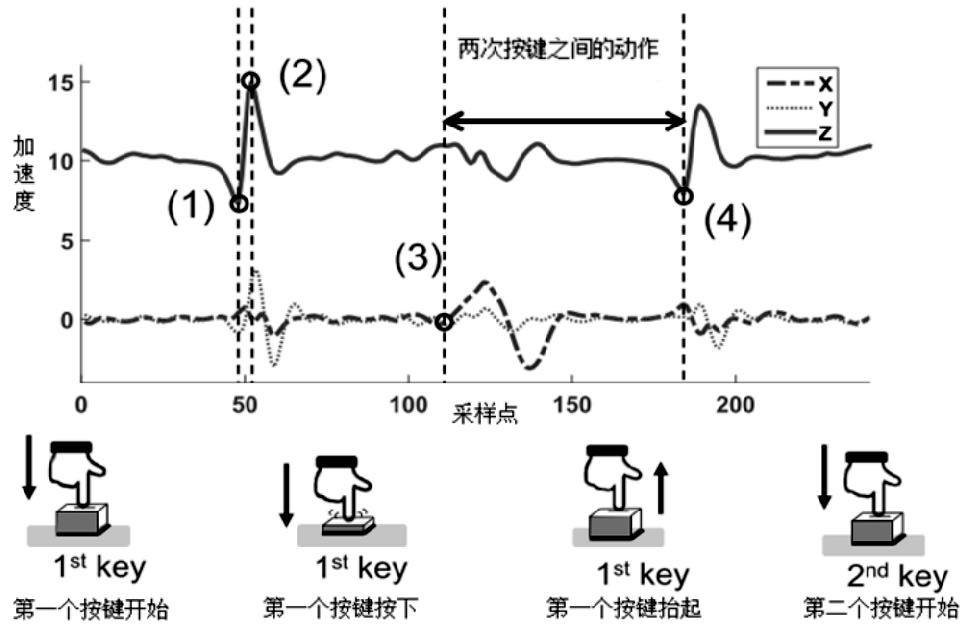
\includegraphics[width=0.7\linewidth]{images/chen.png}
  \caption{加速度传感器数据变化\cite{2018chen}}\label{1-1} % label 用来在文中索引
\end{figure}
\par
{图形密码(如图1-2)是对PIN密码缺点的改进,也是一种通过用户记忆已知密码进行的一种认证方式。研究表明,对比 PIN 码和基于文本的密码,通过手势变化实现的图形密码具有更加易于记忆的优势\cite{ 2008PassShapes},减轻了人的记忆负担,因此在后来的手机用户认证系统中得到了广泛应用。}
\begin{figure}[htbp]
  \centering
  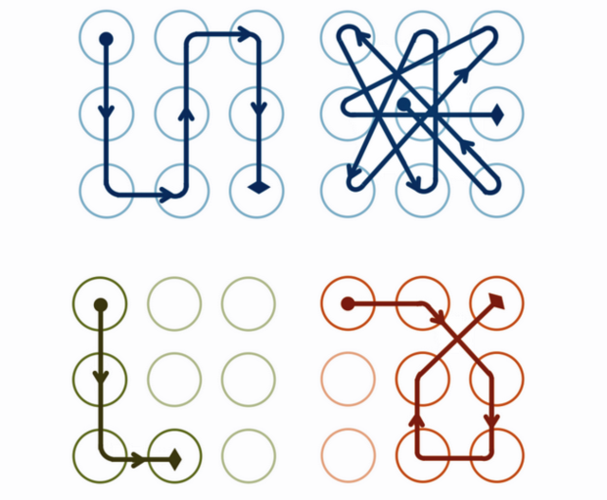
\includegraphics[width=0.5\linewidth]{images/G.jpeg}
  \caption{常见图形密码}\label{1-2} % label 用来在文中索引
\end{figure}
\par
{虽然图形密码在认证系统中克服了PIN码的一些缺点,但是依然是一种基于人脑记忆的已知密码用户认证。它既不能提取用户的生物特征,也不能克服PIN码需要特殊图形或有特殊意义的字母图案来辅助记忆的弊端,同时也不能避免攻击者通过密码测试、密码盗窃、肩膀冲浪\cite{2014Shoulder}、屏幕污迹等方式获取图形密码。更有甚者可以通过监控摄像头获取密码,随着在各种场合监控摄像的广泛分布和清晰度的日益提升,其对个人隐私窃取的隐患也在增加\cite{2022qiu}。对于各种各样的攻击,研究者也在想方设法地应对,文伟平等人实现了一种基于累加方法的防肩窥
图形密码系统\cite{2009wen},通过设计两个不同的密码空间来实现合法用户密码和输入密码不是一一对应,具有较强的随机性,以达到即使攻击者记住用户所有输入密码也无法破解的目的。
}
\par
{即便传统的用户认证系统做出了不少的改进,但是由于这些认证方法都是基于已知密码进行的,始终无法克服记忆繁琐、无法识别生物特征和容易被盗取等缺点,因此在除了PIN码应用于传统认证系统之外,图形密码在智能手机领域的应用以及基本被指纹识别和面容识别取代。}
\subsection{基于生物特征的用户认证}
{为了弥补传统身份认证方法的许多弊端,通过人的生物特征进行系统认证的方法逐渐发展起来,生物特征识别技术(包括个人面部识别特征、指纹、虹膜、声纹等)对比传统的身份认证系统而言,不仅不需要人脑进行密码记忆,而且具有便捷安全的特点\cite{2023he}。在系统优化方面来说,基于生物特征识别的认证方式认证时间缩短,操作方便,而且人的生物特征相对于PIN码和图形密码来说等难以被盗取。随着制造业的发展,一些用于生物特征提取的传感器在智能手机中得到了普及。除此之外,人工智能、大数据领域的发展也为生物特征识别技术提供了理论于技术支持,使得识别、指纹识别、虹膜识别、声纹识别等基于生物特征的认证方式在工业上得到广泛使用。}
\par
{指纹是人类手指末端由凹凸的皮肤所形成的纹路,如图1-3,在人类出生之前指纹就已经形成并且随着个体的成长指纹的形状不会发生改变,只是明显程度的变化,而且每个人的指纹都是不同的,在众多细节描述中能进行良好的区分,在指纹中有许多特征点,特征点提供了指纹唯一性的确认信息,这是进行指纹识别的基础\cite{2019yu}。}
\begin{figure}[htbp]
  \centering
  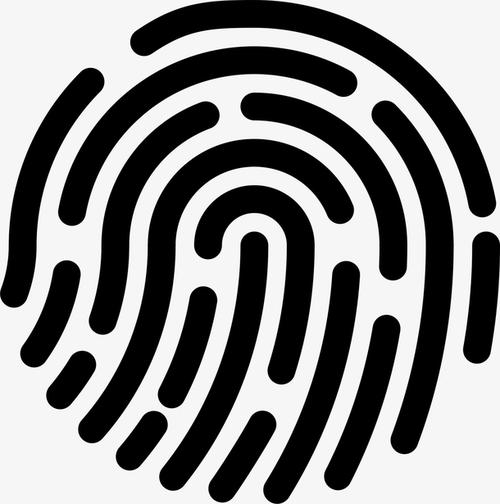
\includegraphics[width=0.2\linewidth]{images/zhi.jpeg}
  \caption{指纹特征}\label{1-3} % label 用来在文中索引
\end{figure}
\par
{指纹识别技术是众多生物特征识别技术中的一种,它需要计算机、数据库、图像处理、人工智能等领域技术的理论支持,还需要智能卡、网络、光电技术等硬件条件的支持。指纹是人们与生俱来的表现在手掌面的遗传学特征,在不受外力强制改变的条件下,指纹具有触物留痕、排列规整、独一无二、终身基本不变等特点,指纹包含的生物特征众多,通过特征点能识别指纹的唯一确认信息\cite{2019yu}。}
\par
{目前指纹识别在智能手机上具有广泛的应用,是一种较为高效、安全的用户认证方式,但是仍有通过特殊指纹提取工具进行攻击的风险。}
\par
{声纹(如图1-4,1-5所示)识别也是是众多生物特征识别技术中的一种,是指通过专用的电声转换仪器将声波特征绘制成波谱图形,与已经注册过的声纹模型对比,从而区分不同的个体,实现身份校验功能。与指纹识别等常见的生物特征识别方式相比,声纹识别具有获取方便自然、使用简单、能远程验证等优点,它同样需要计算机、数据库、人工智能等邻域研究的支持。人在说话时使用的发声器官(舌、牙齿、喉头、肺、鼻腔等)在尺寸和形态方面每个人的差异很大,所以使得任何两个人的声纹图谱都存在差异\cite{2022zhang}。因此在一般情况下,通过声纹识别技术可以区分不同的个体。}
\begin{figure}[htbp]
  \centering
  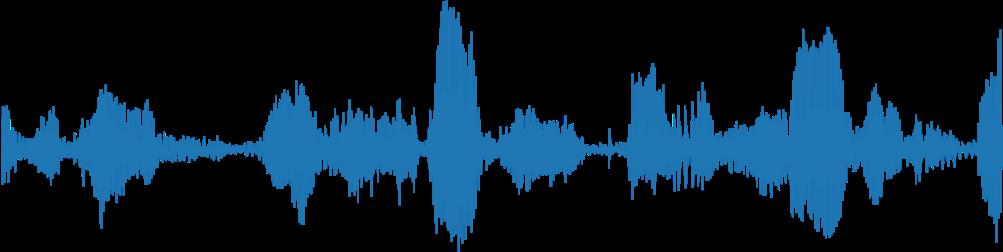
\includegraphics[width=0.5\linewidth]{images/shi.png}
  \caption{声纹时域效果图\cite{2022zhang}}\label{1-4} % label 用来在文中索引
\end{figure}
\begin{figure}[htbp]
  \centering
  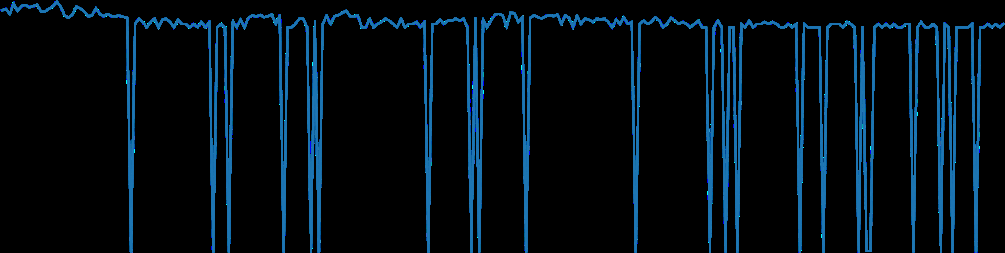
\includegraphics[width=0.5\linewidth]{images/pin.png}
  \caption{声纹频域效果图\cite{2022zhang}}\label{1-5} % label 用来在文中索引
\end{figure}
\par
{声纹技术随着信号处理于人工智能领域的发展,在智能手机上也得到了广泛的应用(如siri、小艺小艺、小爱同学等),但用于身份认证系统,认证过程麻烦,干扰因素较多,没有指纹识别和面容识别方便。除此之外,声纹识别也有被人盗取生物特征的风险,比如对合法用户进行声音录制分析,或者模拟人的发声特点等方式。随着人工智能的快速发展,也出现了AI声音合成等技术。人工智能虽然对生物特征识别领域做出了卓越贡献,但是也产生了对应的攻击方法,增加了安全隐患。}
\par
{面容识别技术也是是众多生物特征识别技术中的一种,是基于人的面容特征信息进行身份认证的一种生物特征识别技术。一般方法是采用摄像头或者摄像机采集包含人的面容信息的图像或者视频流,通过图像处理等技术在图像中检测、跟踪人脸,并获取面容图像,再通过人工智能等技术对提取的面容图像进行训练对比,进而实现对人的面容生物特征进行提取比对,完成用户身份认证的方法(如图1-6所示过程)。通常也叫做人像识别、人脸识别。}
\begin{figure}[htbp]
  \centering
  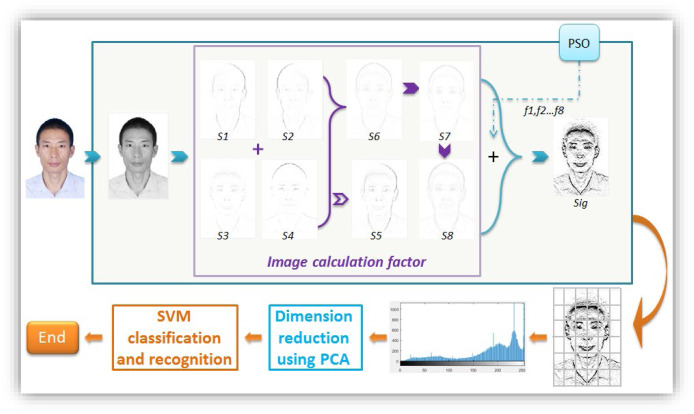
\includegraphics[width=0.8\linewidth]{images/gr4.jpg}
  \caption{人脸识别算法流程图\cite{Song2018Image}}\label{1-6} % label 用来在文中索引
\end{figure}
{与声纹识别、指纹识别等生物特征识别技术相比较,面容识别有更简单、方便、准确等特点,而且使用的传感器为较为传统的摄像头,不像指纹识别一样需要特殊的指纹特征提取传感器来实现,可以应用的范围更广泛\cite{ 2022he}。然而相关面容识别技术的应用也催生了对应的问题,就安全性来说,利用单个人脸图像进行生物特征提取与身份认证会存在非法分子使用合法用户图像进行信息盗取的风险,相对于指纹和声纹,个人面容图像盗取就显得更加容易,因此在商业应用时,一些安全要求较高的邻域一般对用户有眨眼、摇头等动作要求,验证便捷度会有所降低,便捷与安全不可兼得。除此之外,广泛的商业应用也给用户隐私带来了安全隐患,在带来巨大商业利益与便利的同时,用户数据泄露造成的损失也不堪设想\cite{2023yang},因此,相关的法律规范与地方标准的设立至关重要\cite{ 2023ren},对面容识别应用的规范不仅是对用户隐私和利益的保护,也是对行业长远发展的战略布局。}
\subsection{心脏特征的获取与应用}
{高端的智能手机往往配备特殊的生物特征传感器,可以通过识别用户的生物特征来实现用户验证。然而,一些低成本智能手机并不具备该硬件基础。摄像头和一些手机内置的传感器,如麦克风,加速计等都是中高低端设备具有的传感器。Edward JayWang等人设计了实验利用手机加速计和摄像头来测量人的血压\cite{2018Blood}。}
\par
\begin{figure}[htbp]
  \centering
  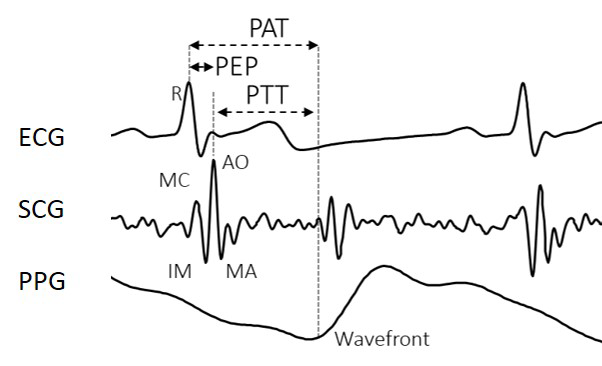
\includegraphics[width=0.5\linewidth]{images/PTT.png}
  \caption{心电曲线(ECG)、震动曲线(SCG)、光体积曲线(PPG)在同一时刻的测量值\cite{2018Blood}}\label{1-7} % label 用来在文中索引
\end{figure}
\par
{具体来说,如图1-7所示,通过手机按压胸部获得的手机加速计数据变化图称为心脏震动描记图(SCG);使用手指按压手机摄像头获取的光强变化图称为光体积描记图(PPG)。心脏震动描记图(SCG)的AO峰出现时记录的是近心端主动脉瓣打开时间;光体积描记图(PPG)的局部极小值,即图1-7中记录的Wavefront,是心脏脉搏到达远心端(手指)的时间。主动脉瓣打开到心脏脉博到达远心端之间的时间称为脉搏传输时间(PTT),人的血压与PTT成正比,Edward JayWang等人通过手机加速计与摄像头来获取PTT并以此估算人的血压。}
\par
{相对于使用图1-7所示的PAT(心电图ECG的R峰出现时间到心脏脉博到达远心端之间的时间)来测量人的血压,PTT具有一些局限性,但是实验\cite{2018Blood}说明通过手指按压摄像头的光体积描记图(PPG)可以获取人的心脏信号,正确描述人的心率、脉搏、血压的变化,并证明了智能手机摄像头捕捉心脏信号的正确性和可行性。}
\par
{除此之外,还有实验表明在大量人群中个体的心脏特征是固有的、独特的\cite{2011Heart,2002Near,2004Feature},说明了心脏特征提取的可能性。但人的心脏信号会受到手指按压位置、人的心理情绪、周围环境、摄像头使用的光学场景不同而受到不同影响,需要通过对提取信息标准化来实现。此外,手指按压的光体积图除了能提取心脏信号外,还能提取用户的皮肤特征,为用户的身份验证提供了额外的生物特征。有实验表明,手指按压的光强度变化在不同的颜色通道中,表现出不同的心脏运动模式,具有独特的心脏特征\cite{2019CardioCam}。由于皮肤特征导致的对不同光线的吸收率不同,导致在不同颜色通道的光强度图中,表现出的用户心脏运动模式的不同为用户特征的独特性提取提供了更为可靠的支持。因此,基于智能手机摄像头的用户身份认证具有实现的可行性和广泛的市场用途。}
\section{主要研究内容}
% 这里插入一个参考文献,仅作参考

	{用户身份认证是保障移动设备(如智能手机、平板电脑)安全的关键环节。本文旨在探索一种低成本且难以伪造的用户身份认证系统,该系统利用智能手机的内置摄像头获取用户指尖按压摄像头的视频帧,并提取用户独特的心脏生物特征进行认证。该系统在智能手机上进行实现,并通过在真实环境中的实验,测试系统验证合法用户、拒绝非法用户的准确性。}

% 一个可能无法正常显示的生僻字
% 一个可能无法正常显示的生僻字: 彧。下文注释中,介绍了如何通过自定义字体来显示生僻字。

% 定义一个提供了生僻字的字体,注意要确保你的系统存在该字体
% \setCJKfamilyfont{custom-font}{Noto Serif CJK SC}

% 使用自己定义的字体
% 使用提供了相应字型的字体:\CJKfamily{custom-font}{彧}。

